\section{The Calorimeters}
\label{sec:calo}

\subsection{Electromagnetic Calorimeter}

Particles that survive the Tracker will then encounter the Electromagnetic Calorimeter (ECAL).
The ECAL is a hermetic homogeneous sub-detector consisting of a barrel part (EB) and two endcap parts (EE).
The EB contains 61200 lead tungstate (PbWO$_4$) crystals while each EE contains 7324 crystals.
Due to its short radiation length (0.89 cm) and high density (8.28 g/cm$^3$),
PbWO$_4$ is a good material to use in the ECAL.
Conveniently after 1 bunch crossing (25 ns), nearly 80\% of the scintillated light is emitted.

\begin{figure*}[!htb]
    \centering
    \captionsetup{justification=justified}
    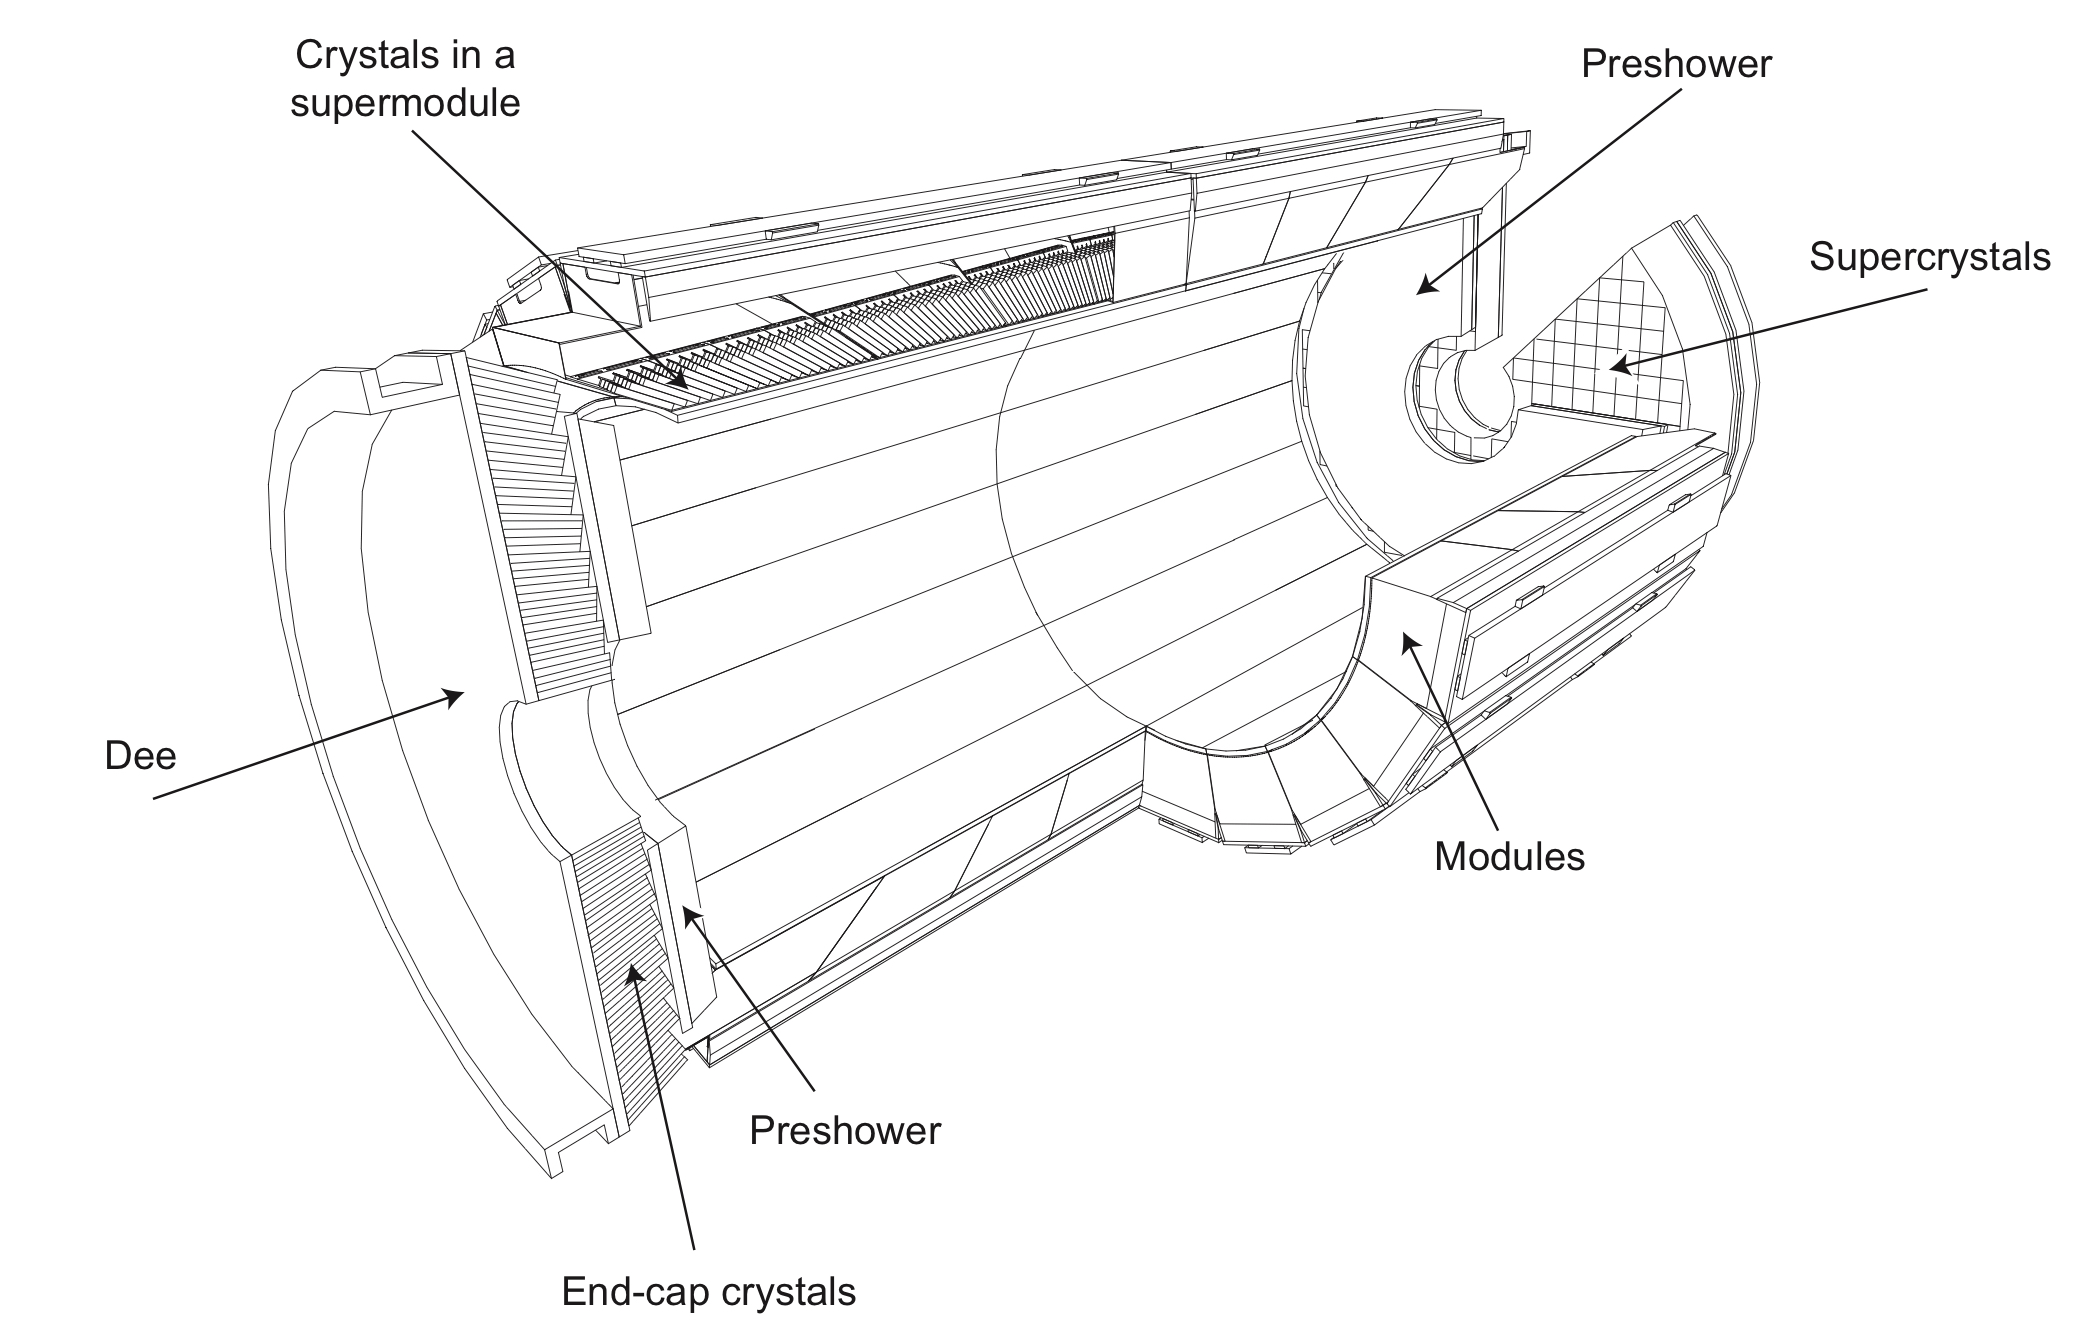
\includegraphics[width=0.95\textwidth]{figures/ECAL/xs_whiteblack.jpeg}
    \caption{Cross sectional view of the electromagnetic calorimeter of CMS.
             Figure taken from Ref.~\cite{jinst:cms_exp}.}
    \label{fig:ecal_xs}
\end{figure*}

whose purpose is to absorb photons and electrons and detect their energies and directions.

%%%%%%%%%%%%%%%%%%
%----- ECAL -----%
%%%%%%%%%%%%%%%%%%
After particles pass through the Silicon Tracker system, they encounter the {\bf Electromagnetic Calorimeter} (ECAL). 
This is a scintillating subdetector made out of approximately 78,000 beautiful, transparent, and heavy ${\rm PbWO_{4}}$ crystals, as shown in Fig.~\ref{fig:ecal_crystals} (Left).
Each crystal weighs 1.5 Kg but has only the volume of a small cup of coffee. 

%%%%%%%%%%%%%%%%%%%%
\begin{figure}[pbth]
\centering
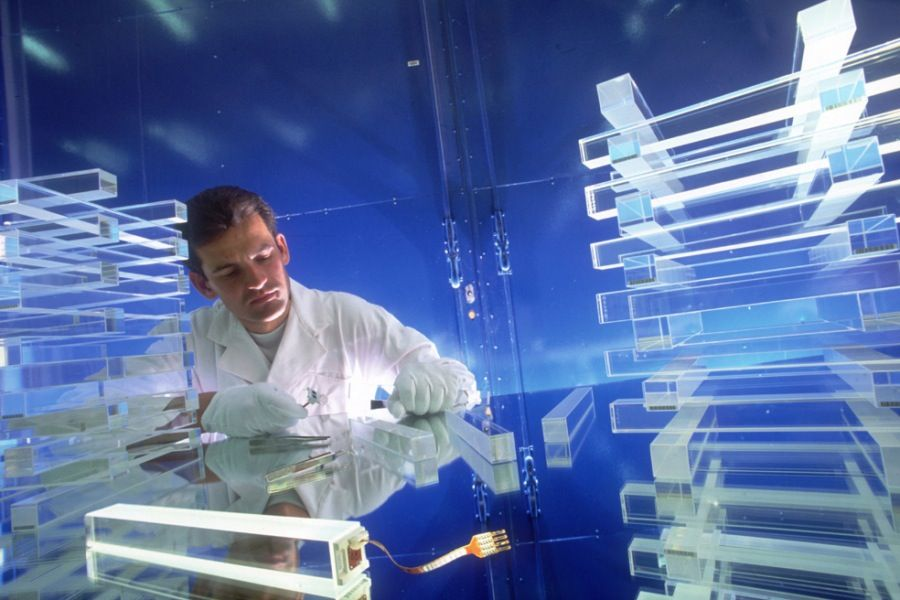
\includegraphics[width=0.49\textwidth,height=10cm,keepaspectratio]{Figures/ECAL_crystals_fancy_lab.jpg}
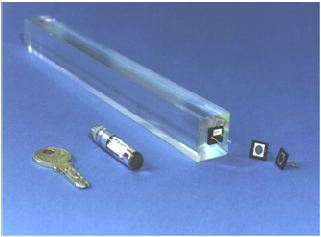
\includegraphics[width=0.49\textwidth,height=10cm,keepaspectratio]{Figures/ECAL_crystal_sizecomparison.jpg}
    \caption{
    (Left) ECAL crystals are grown in a lab.
    (Right) Although made mostly of metal, ECAL crystals are transparent and have a photomultiplier detector attached at the end.} 
    \label{fig:ecal_crystals}
\end{figure}
%%%%%%%%%%%%%%%%%%%%
Electrons and photons interact electromagnetically with the ECAL, creating an electromagnetic (EM) shower, and effectively get trapped here.
The ECAL crystals then give off light (\emph{scintillate}) in proportion to the amount of energy deposited by the electron or photon. 
The scintillator photons are detected by a photomultiplier detector attached to the back of each ECAL crystal (Fig.~\ref{fig:ecal_crystals}, Right).
The ECAL has a barrel component and endcap components.

How does one distinguish between an electron energy deposit in the ECAL system versus and a photon deposit?
The electron will leave hits in the Tracker whereas a photon is electrically neutral and will not generate any signal in the Silicon Tracker. 
So long as the Tracker and ECAL communicate effectively with each other, then they help distinguish between electrons and photons.
Charged hadrons also interact with the ECAL, but only minimally. They very often punch through the ECAL system.
Neutral hadrons can be detected by the ECAL preshower near the ECAL endcaps. 
which helps distinguish a single photon from $\pi^{0}$ mesons as they decay into two photons with a narrow opening angle, making it look as if the two photons are a single photon.

What about those hadrons? They got through the ECAL... To detect hadrons effectively, we need a Hadron Calorimeter.
% That's what we see here with the blue dashed line (the photon) and the red line (the positron).

%%%%%%%%%%%%%%%%%%
%----- HCAL -----%
%%%%%%%%%%%%%%%%%%
\subsection{Hadron Calorimeter}
By the time particles reach the {\bf Hadron Calorimeter} (HCAL), the only kind which remain (usually) are muons and hadrons.
At 1 meter thick, the HCAL is a brass scintillator and its primary purpose is to catch and record the energies of hadrons.
Similar to the ECAL, the HCAL will scintillate in proportion to the amount of energy of the captured particle. 
The incoming hadrons will \emph{hadronize} (\ie, produce a hadronic shower), generating jets of quarks and gluons which are bound in various ways forming protons, neutrons, pions, kaons, \etc.
Interestingly, the HCAL is made using over a million old, brass shell casings from the Russian Navy back from World War II.
% kinds of particles which have not decayed on their own or were not caught by the ECAL, ,  or when it catches hadronic material: stuff made of quarks, like . 

